\section{Algoritmes}

\frame{ \tableofcontents[currentsection] }

\begin{frame}
  \frametitle{Vierkanswortel}
  \structure{Definitie}
  \[
    y = \sqrt{x} \quad\iff\quad y^2 = x
  \]
  \vskip5mm
  \structure{Voorbeelden}
  \[
    \begin{array}{rcl}
      \sqrt1 & = & 1 \\
      \sqrt4 & = & 2 \\
      \sqrt9 & = & 3 \\
             & \vdots & \\
      \sqrt{100} & = & 10 \\
      & \visible<2>{\vdots} \\
      \visible<2>{\sqrt{1000}} & \visible<2>{=} & \visible<2>{?}
    \end{array}
  \]
\end{frame}


\begin{frame}
  \frametitle{Vierkantswortel}
  \code[font size=\small,width=.95\linewidth]{sqrt.js}
\end{frame}

\begin{frame}
  \frametitle{Algorithms: They're Everywhere}
  \begin{center}
    \begin{tikzpicture}[box/.style={fill=red,opacity=.25,ultra thick},
                        msg/.style={rectangle,fill=red,opacity=.25,text opacity=1}]
      \path[use as bounding box] (-5,-1) rectangle (5,5);
      \node[anchor=south] (pic) at (0,0) { \pgfimage[width=10cm,interpolate=true]{borderlands.jpg} };
      \only<2>{
        \draw[box] (1, 4.5) circle (1);
        \node[msg,anchor=north] at (0, 0) { \parbox{10cm}{ \centering
            Hidden surface removal \\ {\tiny (Z-buffering, Painter's Algorithm, BSP trees, \dots)}
        }};
      }
      \only<3>{
        \draw[box] (-3, 3) circle (1);
        \draw[box] (1.5, 3) circle (.5);
        \node[msg,anchor=north] at (0, 0) { \parbox{10cm}{ \centering
            Hit detection
        }};
      }
      \only<4>{
        \draw[box] (1.85, 2.3) circle (.75);
        \node[msg,anchor=north] at (0, 0) { \parbox{10cm}{ \centering
            Particle system (fire simulation)
        }};
      }
      \only<5>{
        \draw[box] (0, 2) circle (.9);
        \draw[box] (3.5, 1.2) circle (.9);
        \node[msg,anchor=north] at (0, 0) { \parbox{10cm}{ \centering
            Shadow casting (static vs dynamic)
        }};
      }
      \only<6>{
        \draw[box] (0.3, 2.7) circle (.5);
        \node[msg,anchor=north] at (0, 0) { \parbox{10cm}{ \centering
            Artificial Intelligence \\
            {\tiny (Path Finding: A-star, Game Trees: Minimax, Artifical Neural Networks, \dots)}
        }};
      }
    \end{tikzpicture}
  \end{center}
\end{frame}

\begin{frame}
  \frametitle{Algoritmes}
  \begin{itemize}
    \item Stap-voor-stap beschrijving van oplossingsmethode
          \vskip5mm
    \item Drie ``kwaliteitsmetrieken''
          \begin{itemize}
            \item Algoritme moet ooit eindigen
            \item Algoritme moet correct resultaat opleveren
            \item Algoritme moet zo effici\"ent mogelijk werken
          \end{itemize}
          \vskip5mm
    \item Knelpunten
          \begin{itemize}
            \item Enige creativiteit vereist
            \item Randgevallen
            \item Begrijpen van de details
          \end{itemize}
  \end{itemize}
\end{frame}

\begin{frame}
  \frametitle{Puzzel}
  \begin{center}
    \begin{tikzpicture}
      \node { \pgfimage[width=5cm,interpolate=true]{scale.png} };
    \end{tikzpicture}
  \end{center}  
  \begin{overprint}
    \onslide<1>
    \structure{Probleemstelling}
    \begin{itemize}
      \item Gegeven 9 identiek uitziende goudmunten
      \item E\'en ervan is vals, deze is wat lichter
      \item Vind de valse munt met zo weinig mogelijk wegingen
    \end{itemize}

    \onslide<2>
    \structure{Na\"ieve oplossing}
    \begin{itemize}
      \item Telkens twee munten met elkaar vergelijken
      \item Een lichtere gevonden $\rightarrow$ valse munt gevonden
      \item Kan tot 7 wegingen leiden
    \end{itemize}

    \onslide<3>
    \structure{Effici\"entste oplossing}
    \begin{itemize}
      \item Drie munten met drie andere vergelijken
      \item Indien gelijk: valse zit in laatste drie
      \item Anders: kies de lichtste drie
      \item Slechts 2 wegingen nodig
    \end{itemize}

  \end{overprint}
\end{frame}

\begin{frame}
  \frametitle{Overzicht Cursus}
  \begin{enumerate}
    \item Variabelen
    \item Conditionele Logica
    \item Lussen
    \item Functies
    \item Recursie
    \item Rijen
    \item Sorteeralgoritmen
    \item Complexiteit
  \end{enumerate}
\end{frame}


%%% Local Variables: 
%%% mode: latex
%%% TeX-master: "intro"
%%% End: 
